\documentclass{beamer}
\usepackage[utf8]{inputenc}
\usetheme{Madrid}
\usecolortheme{default}
\usepackage{amsmath,amssymb,amsfonts,amsthm}
\usepackage{txfonts}
\usepackage{tkz-euclide}
\usepackage{listings}
\usepackage{adjustbox}
\usepackage{array}
\usepackage{tabularx}
\usepackage{gvv}
\usepackage{lmodern}
\usepackage{circuitikz}
\usepackage{tikz}
\usepackage{graphicx}

\setbeamertemplate{page number in head/foot}[totalframenumber]

\usepackage{tcolorbox}
\tcbuselibrary{minted,breakable,xparse,skins}



\definecolor{bg}{gray}{0.95}
\DeclareTCBListing{mintedbox}{O{}m!O{}}{%
  breakable=true,
  listing engine=minted,
  listing only,
  minted language=#2,
  minted style=default,
  minted options={%
    linenos,
    gobble=0,
    breaklines=true,
    breakafter=,,
    fontsize=\small,
    numbersep=8pt,
    #1},
  boxsep=0pt,
  left skip=0pt,
  right skip=0pt,
  left=25pt,
  right=0pt,
  top=3pt,
  bottom=3pt,
  arc=5pt,
  leftrule=0pt,
  rightrule=0pt,
  bottomrule=2pt,
  toprule=2pt,
  colback=bg,
  colframe=orange!70,
  enhanced,
  overlay={%
    \begin{tcbclipinterior}
    \fill[orange!20!white] (frame.south west) rectangle ([xshift=20pt]frame.north west);
    \end{tcbclipinterior}},
  #3,
}
\lstset{
    language=C,
    basicstyle=\ttfamily\small,
    keywordstyle=\color{blue},
    stringstyle=\color{orange},
    commentstyle=\color{green!60!black},
    numbers=left,
    numberstyle=\tiny\color{gray},
    breaklines=true,
    showstringspaces=false,
}
%------------------------------------------------------------
%This block of code defines the information to appear in the
%Title page
\title %optional
{3.4.6}

%\subtitle{A short story}

\author % (optional)
{stalin-ai25btech11037}



\begin{document}


\frame{\titlepage}
\begin{frame}{Question}
Construct a rhombus whose diagonals are \(4 \, \text{cm}\) and \(6 \, \text{cm}\) in lengths.\\ 
\end{frame}
\begin{frame}{Theoretical Solution}
Let us solve the given equation theoretically and then verify the solution computationally \\
According to the question, \\
Given $D_1$=\(4 \, \text{cm}\) $D_2$=\(6 \, \text{cm}\)\\
Let centre be $\vec{O}$ 
\begin{align}
  \vec{O}=\begin{myvec}{0\\0}\end{myvec}\;
  \end{align}
points be
  \begin{align}
  \vec{A}=\begin{myvec}{2\\0}\end{myvec}\;
  \vec{B}=\begin{myvec}{3\\0}\end{myvec}\;
\vec{C}=\begin{myvec}{-2\\0}\end{myvec}\
  \vec{D}=\begin{myvec}{-3\\0}\end{myvec}\
   \end{align}
\end{frame}
\begin{frame}[fragile]
    \frametitle{python code }
    \begin{lstlisting}
   import matplotlib.pyplot as plt

# Vertices of rhombus (centered at origin)
A = (-3, 0)
B = (0, 2)
C = (3, 0)
D = (0, -2)

# Collect points to plot closed rhombus
x = [A[0], B[0], C[0], D[0], A[0]]
y = [A[1], B[1], C[1], D[1], A[1]]

# Plot rhombus
plt.figure(figsize=(6,6))
plt.plot(x, y, 'b-o', linewidth=2)
plt.fill(x, y, 'skyblue', alpha=0.5)










    \end{lstlisting}
\end{frame}
\begin{frame}[fragile]
    \frametitle{python code }
    \begin{lstlisting}
# Mark vertices
plt.text(A[0]-0.3, A[1], "A(-3,0)", fontsize=12)
plt.text(B[0], B[1]+0.3, "B(0,2)", fontsize=12, ha="center")
plt.text(C[0]+0.3, C[1], "C(3,0)", fontsize=12)
plt.text(D[0], D[1]-0.3, "D(0,-2)", fontsize=12, ha="center")

# Add diagonals
plt.plot([-3, 3], [0, 0], 'r--')  # horizontal diagonal
plt.plot([0, 0], [-2, 2], 'r--')  # vertical diagonal

# Styling
plt.title("Rhombus with diagonals 4 cm and 6 cm")
plt.axis("equal")
plt.grid(True)
# Save figure
plt.savefig("rhombus.png", dpi=300)
plt.show()

\end{lstlisting}
\end{frame}

\begin{frame}[fragile]
    \frametitle{python code }
    \begin{lstlisting}
# Labels
ax.set_xlabel('X-axis')
ax.set_ylabel('Y-axis')
ax.set_zlabel('Z-axis')
ax.set_title(f"Distance between planes = {distance:.2f}")

# Save figure
plt.savefig("planes_distance.png", dpi=300)
plt.show()

    \end{lstlisting}
\end{frame}
\begin{frame}{Plot}
    \centering
    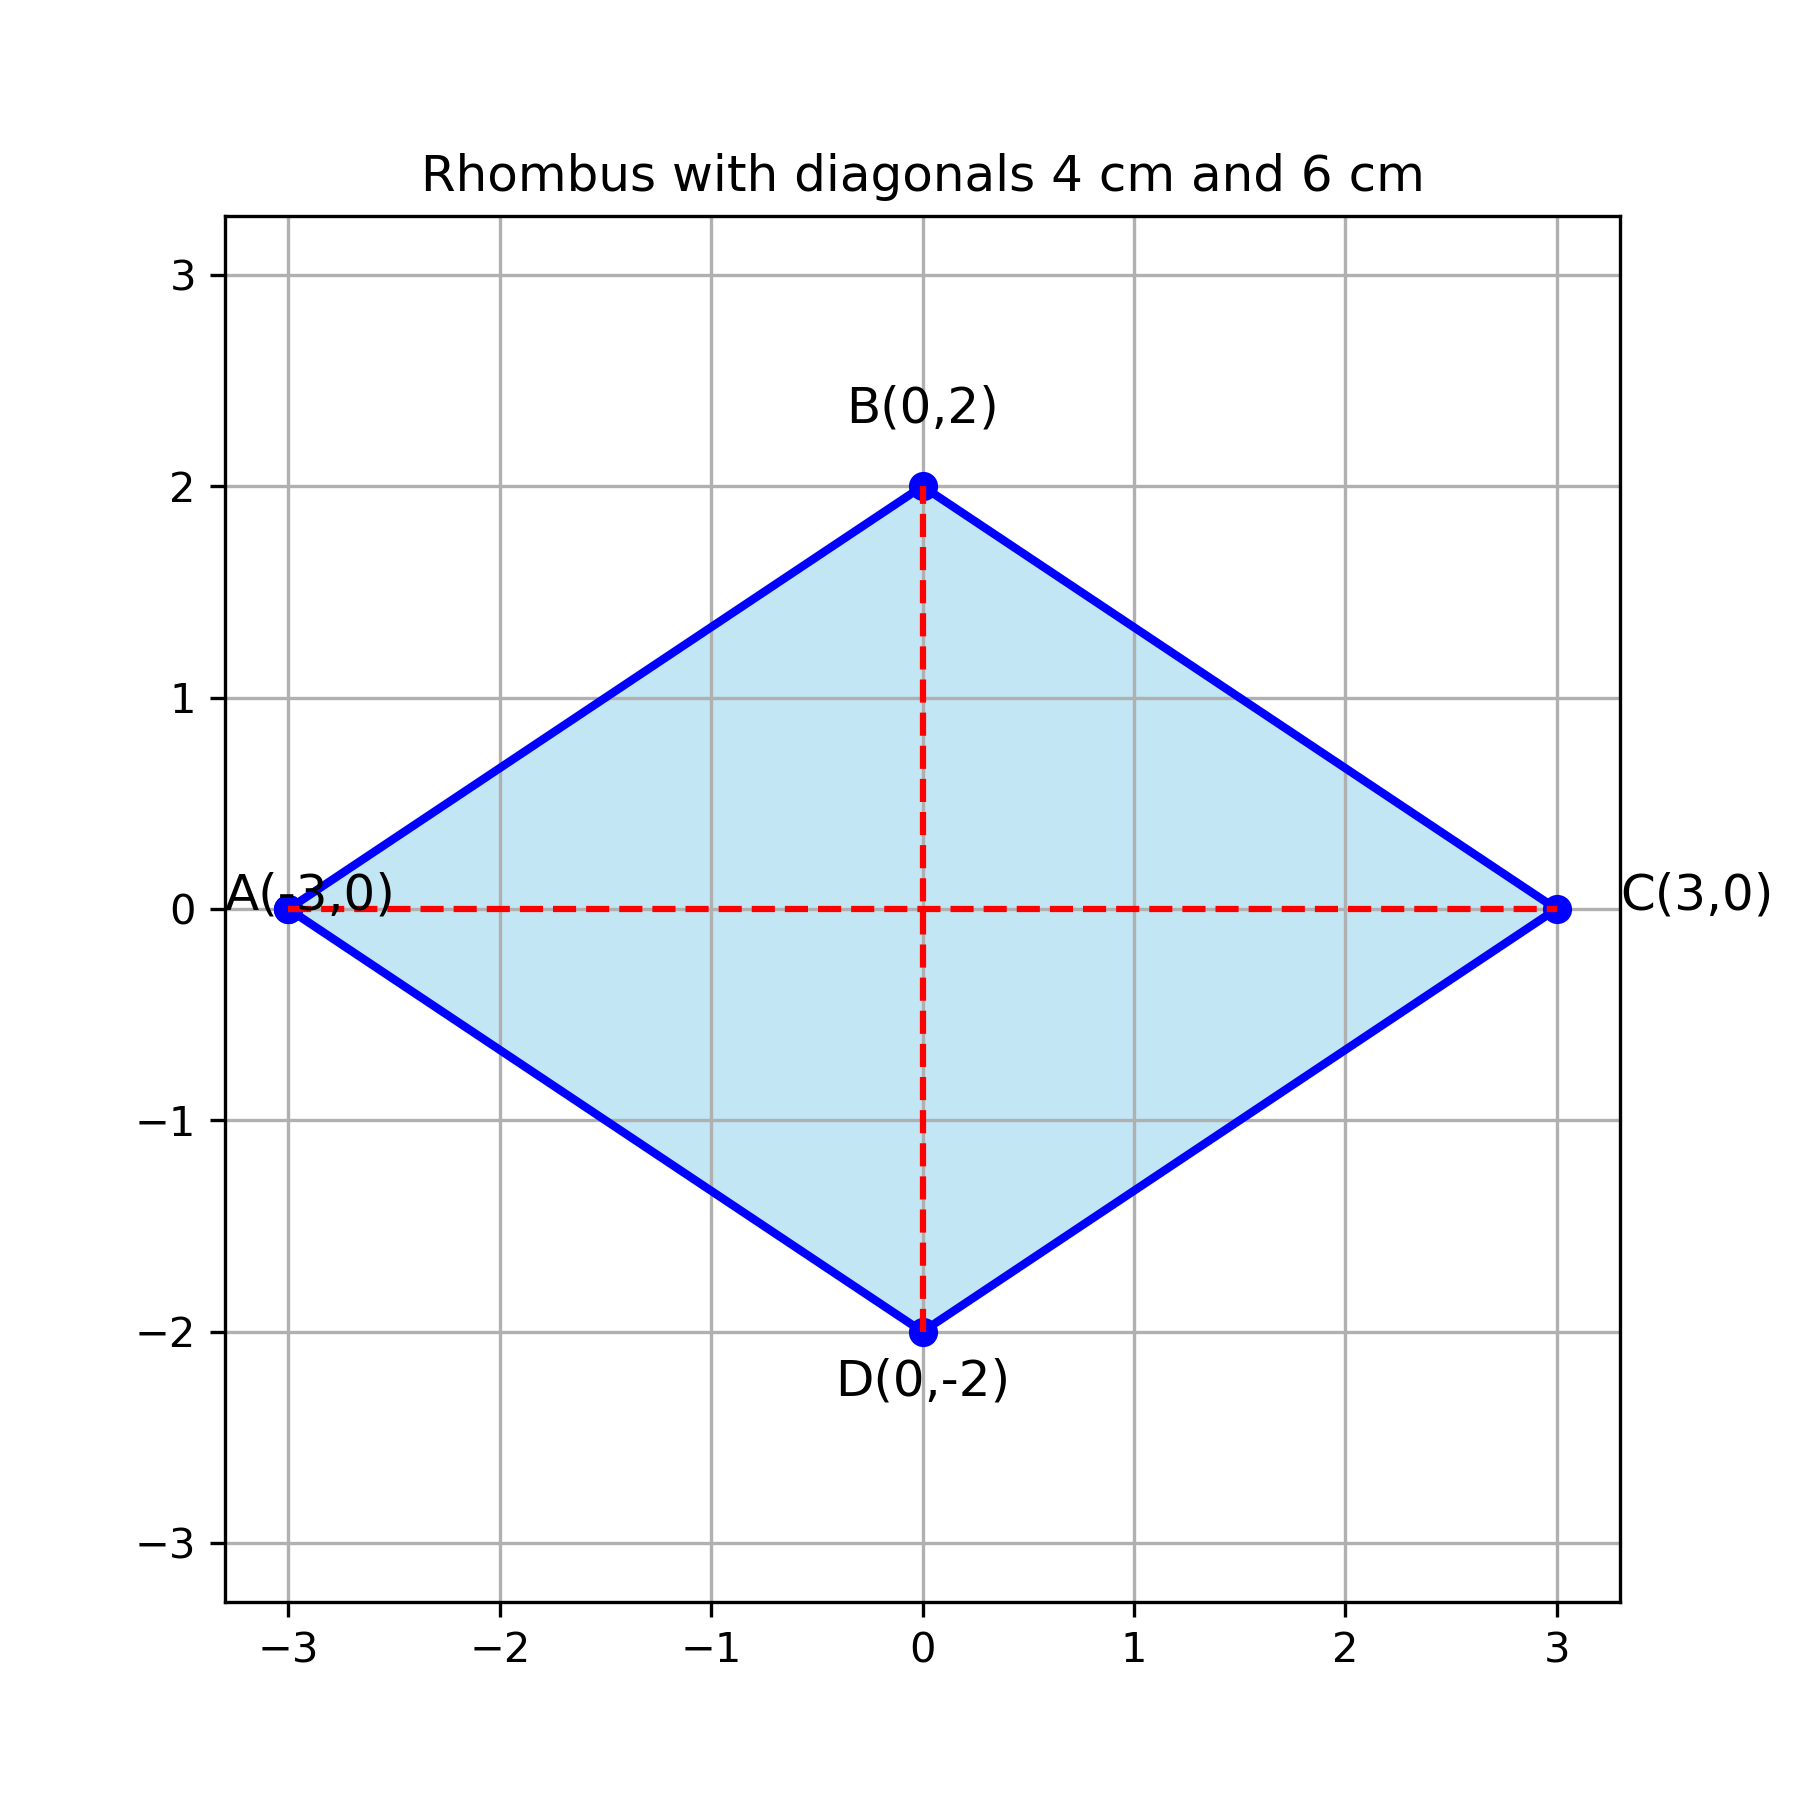
\includegraphics[width=\columnwidth, height=0.8\textheight, keepaspectratio]{figs/rhombus.png}     
\end{frame}

\end{document}